\documentclass[aspectratio=43]{beamer}
\usepackage[utf8]{inputenc}
\usepackage{beamer_eit-en}
\usepackage{lmodern}
\usepackage{graphicx}
\usepackage[backend=biber, style=ieee, sorting=nyt]{biblatex}
\usepackage[font=small, justification=centering]{caption}
\usepackage{lipsum}


\usepackage[absolute,overlay]{textpos} %for proper textpositioning

% Correctly display SI units
\usepackage{siunitx}
\DeclareSIUnit{\rpm}{rpm}

\renewcommand{\footnotesize}{\scriptsize}
\renewcommand*{\thefootnote}{[\arabic{footnote}]}

\newcommand{\picref}[1]{{%
  \let\thempfn\relax% Remove footnote number printing mechanism
  \footnotetext[0]{\emph{#1}}% Print footnote text
}}

\addbibresource{references.bib}

\title[Scientific Working]{Musical neurofeedback for treating depression in elderly people}
\subtitle{Rafael Ramirez, Manel Palencia-Lefler, Sergio Giraldo and Zacharias Vamvakousis}
\author{Presented by Kymbat Talant}

\institute[OVGU FEIT]{
	Faculty of Electrical Engineering and Information Technology,\\
        Otto-von-Guericke-Universität, Magdeburg
}
\mode<presentation>{\keywords{Schlüsselwörter durch Komma getrennt}}
\date[19.06.2018]%{Datum der Präsentation, \zB 1. Januar 2016}

\begin{document}

\begin{frame}
        \maketitle
        % \maketitle funktioniert auch im Article-Modus^M
        % \titlepage funktioniert nur bei Präsentationen^M
\end{frame}

\begin{frame}{Table of contents}
       \tableofcontents
\end{frame}

\section{Introduction}
\begin{frame}{Introduction}
	\begin{figure}
	\includegraphics[width=0.8\linewidth]{./figures/-004.jpg}
	\caption{ Neurofeedback system Overview}
	\end{figure}
	\picref{\scriptsize{\fullcite{musical}}}
\end{frame}

\begin{frame}{Combination of music (therapy), neurofeedback and emotion detection}
	\begin{figure}
	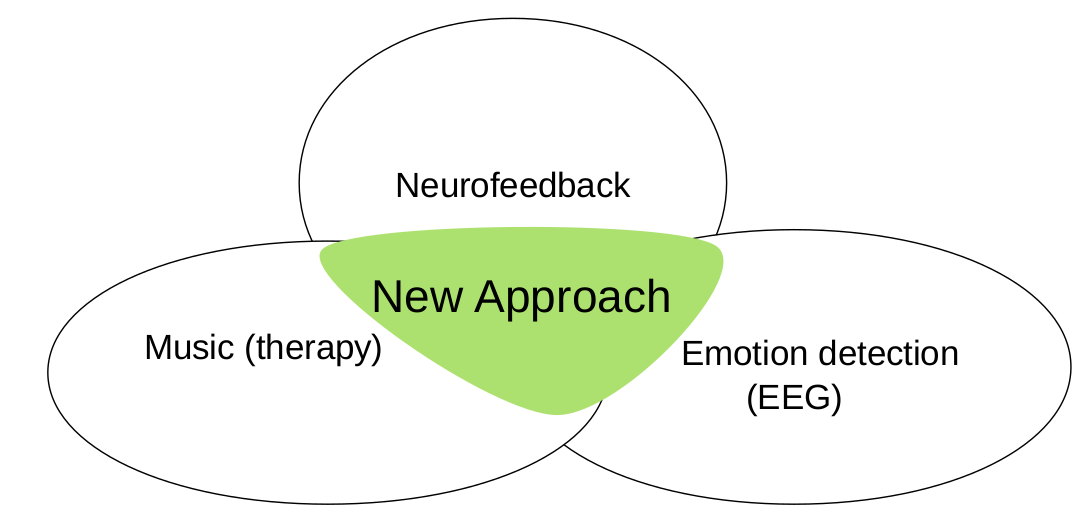
\includegraphics[width=0.8\linewidth]{./figures/New_Approach.png}
	\caption{New Approach for improving elderly people's mental health}
	\end{figure}
\end{frame}

\begin{frame}{Neurofeedback}
Field of applications
\begin{itemize}
\item Depression
\item Anxiety
\item Migraine
\item Epilepsy
\item Attention deficit /hyperactivity disorder
\item alcoholism
\item Chronic pain
\end{itemize}
\end{frame}

\section{Materials and Methods}



\begin{frame}{Table of Contents}
	\tableofcontents[currentsection]
\end{frame}
  

\section{Results}

\begin{frame}{Table of Contents}
	\tableofcontents[currentsection]
\end{frame}



\section{Discussion}

\begin{frame}{Table of Contents}
	\tableofcontents[currentsection]
\end{frame}



\section{Conclusion}

\begin{frame}{Table of Contents}
	\tableofcontents[currentsection]
\end{frame}

\end{document}
